\documentclass[aspectratio=169]{beamer}
\usepackage[T1]{fontenc}
\usepackage[utf8]{inputenc}
\usepackage{lmodern}
\usepackage{microtype}
\usepackage{xcolor}
\usepackage{tikz}
\usetikzlibrary{positioning, arrows.meta, calc}
\usepackage{fontawesome5}
\definecolor{wurgreen}{HTML}{34B233}
\definecolor{darkgreen}{HTML}{1F6B1E}
\definecolor{darknavy}{HTML}{1A1A2E}
\definecolor{midgray}{HTML}{6B7280}
\definecolor{lightgray}{HTML}{F3F4F6}
\definecolor{lightgreen}{HTML}{E8F7E8}
\definecolor{bodytext}{HTML}{1F2937}
\definecolor{warnred}{HTML}{FEE2E2}
\definecolor{warnborder}{HTML}{EF4444}
\definecolor{codebg}{HTML}{1E1E2E}
\definecolor{codegreen}{HTML}{9ECE6A}
\definecolor{codeblue}{HTML}{7AA2F7}
\definecolor{codeorange}{HTML}{FF9E64}
\definecolor{codegray}{HTML}{C0CAF5}
\usetheme{default}\usecolortheme{default}\usefonttheme{professionalfonts}
\setbeamertemplate{navigation symbols}{}
\setbeamertemplate{itemize items}{\textcolor{wurgreen}{\textbullet}}
\setbeamertemplate{itemize subitem}{\textcolor{midgray}{--}}
\setbeamercolor{frametitle}{fg=white, bg=darknavy}
\setbeamerfont{frametitle}{size=\large, series=\bfseries}
\setbeamertemplate{frametitle}{%
  \begin{beamercolorbox}[wd=\paperwidth, ht=1.1cm, dp=0.2cm, leftskip=0.6cm]{frametitle}
    \usebeamerfont{frametitle}\insertframetitle\end{beamercolorbox}}
\setbeamercolor{background canvas}{bg=white}
\setbeamercolor{normal text}{fg=bodytext}
\setbeamertemplate{footline}{%
  \begin{beamercolorbox}[wd=\paperwidth, ht=0.4cm, dp=0.15cm]{footline}
    \hspace{0.5cm}\textcolor{midgray}{\tiny Introduction to Python · Module 4: Functions}%
    \hfill\textcolor{midgray}{\tiny \insertframenumber}\hspace{0.4cm}\end{beamercolorbox}}
\newcommand{\codebox}[1]{\begin{center}
  \begin{tikzpicture}\node[fill=codebg, rounded corners=4pt, inner sep=9pt, text width=0.85\textwidth, text=codegray]{\ttfamily\small #1};\end{tikzpicture}\end{center}}
\begin{document}
{\setbeamertemplate{footline}{}
\begin{frame}[plain]
  \begin{tikzpicture}[remember picture, overlay]
    \fill[darknavy] (current page.south west) rectangle (current page.north east);
    \fill[wurgreen] (current page.south west) rectangle ([xshift=0.45cm]current page.north west);
    \node[anchor=west, text=white, font=\huge\bfseries, text width=13cm] at ([xshift=1.1cm, yshift=1.4cm]current page.west){Introduction to Python};
    \node[anchor=west, text=wurgreen, font=\large, text width=12cm] at ([xshift=1.1cm, yshift=0.2cm]current page.west){Module 4 --- Functions};
    \node[anchor=west, text=midgray, font=\small, text width=12cm] at ([xshift=1.1cm, yshift=-1.3cm]current page.west){Functions, scope, and list comprehensions};
  \end{tikzpicture}
\end{frame}}

\begin{frame}{Why Functions?}
\vspace{0.2cm}
{\small A \textbf{function} is a reusable block of code with a name. Instead of copying the same
lines everywhere, you write them once and \textbf{call} the function whenever you need it.}
\medskip
\begin{columns}[T]
  \column{0.48\textwidth}\vspace{0pt}
  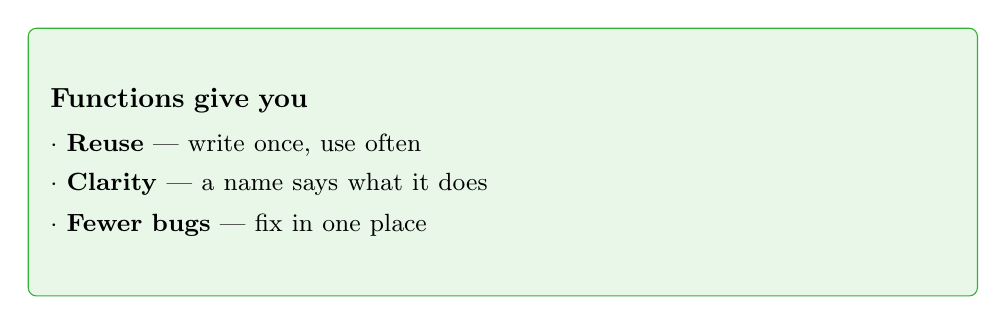
\begin{tikzpicture}
    \node[fill=lightgreen, draw=wurgreen, rounded corners=3pt, inner xsep=8pt, inner ysep=8pt, text width=\columnwidth-18pt, minimum height=3.4cm]{%
      \textbf{Functions give you}\\[5pt]
      {\small
      $\cdot$ \textbf{Reuse} --- write once, use often\\[3pt]
      $\cdot$ \textbf{Clarity} --- a name says what it does\\[3pt]
      $\cdot$ \textbf{Fewer bugs} --- fix in one place}};
  \end{tikzpicture}
  \column{0.48\textwidth}\vspace{0pt}
  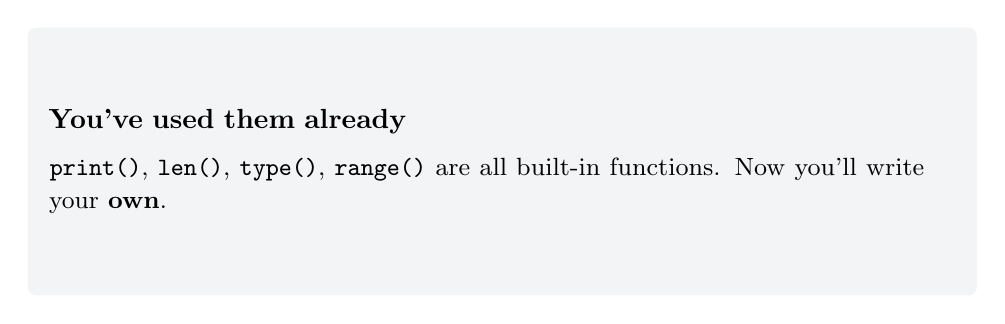
\begin{tikzpicture}
    \node[fill=lightgray, rounded corners=3pt, inner xsep=8pt, inner ysep=8pt, text width=\columnwidth-18pt, minimum height=3.4cm]{%
      \textbf{You've used them already}\\[5pt]
      {\small
      \texttt{print()}, \texttt{len()}, \texttt{type()}, \texttt{range()} are all built-in
      functions. Now you'll write your \textbf{own}.}};
  \end{tikzpicture}
\end{columns}
\end{frame}

\begin{frame}{Defining a Function}
\vspace{0.2cm}
{\small Use \texttt{def}, a name, \textbf{parameters} in parentheses, and \texttt{return} to send
back a result.}
\medskip
\codebox{%
\textcolor{codeblue}{def} greet(name):\\
\quad message \textcolor{codegray}{=} \textcolor{codeblue}{f}\textcolor{codegreen}{"Hello, \{name\}!"}\\
\quad\textcolor{codeblue}{return} message\\[8pt]
\textcolor{codegray}{\# call it}\\
greet(\textcolor{codegreen}{"Denise"})\quad\textcolor{codegray}{\# "Hello, Denise!"}}
\medskip
{\small \texttt{name} is a \textbf{parameter} --- a placeholder filled in when you call the
function. \texttt{return} hands back the result so you can use it.}
\end{frame}

\begin{frame}{Arguments \& Return Values}
\vspace{0.2cm}
{\small Functions can take \textbf{several arguments}, and give them \textbf{default values}.}
\medskip
\codebox{%
\textcolor{codeblue}{def} power(base, exponent\textcolor{codegray}{=}\textcolor{codeorange}{2}):\\
\quad\textcolor{codeblue}{return} base \textcolor{codegray}{**} exponent\\[8pt]
power(\textcolor{codeorange}{5})\quad\ \ \ \ \textcolor{codegray}{\# 25  (exponent defaults to 2)}\\
power(\textcolor{codeorange}{5}, \textcolor{codeorange}{3})\quad\ \textcolor{codegray}{\# 125 (override the default)}\\
power(\textcolor{codeorange}{2}, exponent\textcolor{codegray}{=}\textcolor{codeorange}{10})\quad\textcolor{codegray}{\# 1024 (name the argument)}}
\medskip
{\small A function \textbf{without} a \texttt{return} gives back \texttt{None}. A function can
return \emph{any} type --- a number, a string, a list, a dictionary\ldots}
\end{frame}

\begin{frame}{Scope: Variables Live Inside}
\vspace{0.2cm}
{\small Variables created \emph{inside} a function exist only there --- this is called
\textbf{scope}. It keeps functions self-contained and prevents accidental clashes.}
\medskip
\codebox{%
\textcolor{codeblue}{def} add(a, b):\\
\quad result \textcolor{codegray}{=} a \textcolor{codegray}{+} b\quad\textcolor{codegray}{\# 'result' lives only in here}\\
\quad\textcolor{codeblue}{return} result\\[8pt]
add(\textcolor{codeorange}{2}, \textcolor{codeorange}{3})\quad\ \textcolor{codegray}{\# 5}\\
\textcolor{codeblue}{print}(result)\quad\textcolor{codegray}{\# ERROR - 'result' doesn't exist out here}}
\medskip
{\small\textcolor{midgray}{\textit{Think of a function as a room: what happens inside stays
inside, unless you \texttt{return} it out.}}}
\end{frame}

\begin{frame}{List Comprehensions}
\vspace{0.2cm}
{\small A compact, very ``Pythonic'' way to build a list by transforming another. It replaces a
whole \texttt{for} loop with one readable line.}
\medskip
\codebox{%
words \textcolor{codegray}{=} [\textcolor{codegreen}{"cat"}, \textcolor{codegreen}{"dog"}, \textcolor{codegreen}{"bird"}]\\[6pt]
\textcolor{codegray}{\# the long way}\\
lengths \textcolor{codegray}{=} []\\
\textcolor{codeblue}{for} w \textcolor{codeblue}{in} words:\\
\quad lengths.\textcolor{codeblue}{append}(\textcolor{codeblue}{len}(w))\\[6pt]
\textcolor{codegray}{\# the comprehension way -- same result}\\
lengths \textcolor{codegray}{=} [\textcolor{codeblue}{len}(w) \textcolor{codeblue}{for} w \textcolor{codeblue}{in} words]\quad\textcolor{codegray}{\# [3, 3, 4]}}
\medskip
{\small You can add a condition too: \texttt{[w for w in words if len(w) > 3]} keeps only long
words. Comprehensions are everywhere in real Python.}
\end{frame}

\begin{frame}{Module 4: Takeaways}
\vspace{0.3cm}
\begin{itemize}\setlength\itemsep{8pt}
  \item[\textcolor{wurgreen}{\faCheck}] \texttt{def name(params):} defines a reusable function
  \item[\textcolor{wurgreen}{\faCheck}] \texttt{return} sends a result back; no return means \texttt{None}
  \item[\textcolor{wurgreen}{\faCheck}] Arguments can have \textbf{defaults} and be passed \textbf{by name}
  \item[\textcolor{wurgreen}{\faCheck}] Variables inside a function have local \textbf{scope}
  \item[\textcolor{wurgreen}{\faCheck}] \textbf{List comprehensions} \texttt{[f(x) for x in xs]} build lists compactly
\end{itemize}
\medskip
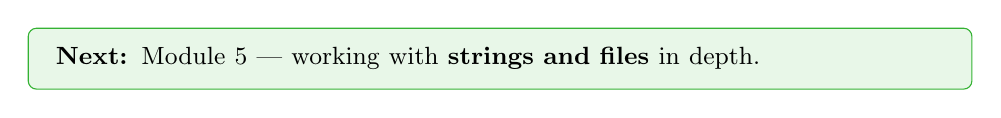
\begin{tikzpicture}
  \node[fill=lightgreen, draw=wurgreen, rounded corners=3pt, inner xsep=10pt, inner ysep=7pt, text width=\textwidth-24pt]{%
    {\small \textbf{Next:} Module 5 --- working with \textbf{strings and files} in depth.}};
\end{tikzpicture}
\end{frame}
\end{document}
